\section*{Anexo D. Importación de un cruce desde OpenStreetMap}

\section{Instalación y configuración de SUMO}

\begin{enumerate}
  \item \textbf{Descargar e instalar SUMO.} Obtenga la versión estable
    de SUMO desde el sitio oficial y siga las instrucciones de
    instalación para su sistema operativo.  SUMO incluye varios
    ejecutables de consola, como \emph{sumo} (simulación),
    \emph{sumo-gui} (versión con interfaz gráfica) y
    \emph{netconvert} (importación de redes).
    Instale también Python~3, necesario para ejecutar los
    scripts auxiliares.

  \item \textbf{Configurar el entorno.} Defina la variable de
    entorno \verb|SUMO_HOME| apuntando al directorio donde se instaló
    SUMO y añada la carpeta \verb|bin| al \verb|PATH| del sistema.
    Esto permite invocar los programas de SUMO desde cualquier
    terminal.

  \item \textbf{Verificar la instalación.} Abra una terminal y ejecute
    los siguientes comandos.  Deben devolver la versión instalada de
    SUMO para confirmar que el entorno está listo:

    {\footnotesize\begin{verbatim}
sumo -V
sumo-gui -V
    \end{verbatim}
    }
\end{enumerate}


%----------------------------------------------------------------------
\section{Limpieza y configuración del escenario OSM \texorpdfstring{$\rightarrow$}{a} SUMO}
\label{sec:osm-limpieza}

Cuando la red proviene de cartografía real, es necesario revisar y
ajustar el escenario para que represente fielmente la intersección de
estudio y resulte adecuado para el entrenamiento del agente de control.
Este proceso consiste en eliminar elementos irrelevantes, corregir
inconsistencias topológicas y configurar adecuadamente los semáforos y
la demanda. El procedimiento que sigue es el previsto para el cruce
real de Lima; los cinco escenarios evaluados en esta fase se
construyeron por el camino alternativo descrito en la
Sección~\ref{sec:escenarios}, escribiendo directamente los archivos de
nodos y vías, por lo que no requirieron limpieza. Las figuras de esta
sección ilustran el procedimiento sobre una intersección de ejemplo y
no corresponden a ninguno de los escenarios evaluados.

\subsection*{Eliminación y simplificación de la red}

\begin{enumerate}
  \item \textbf{Abrir la red en un editor.} Utilice \verb|sumo-gui| o
    \texttt{netedit}, las herramientas de SUMO destinadas a la
    inspección y edición de redes. Desde la interfaz gráfica se puede
    seleccionar manualmente cada calle, carril e intersección para
    examinar su geometría y atributos.

  \item \textbf{Eliminar calles irrelevantes.} Desactive o borre los
    segmentos de vía que no formen parte del cruce objeto de estudio.
    En \texttt{netedit} esto puede realizarse en modo ``Edge''
    seleccionando los elementos y pulsando la tecla Suprimir. También
    se pueden modificar jerarquías de carreteras para mantener
    únicamente arterias principales y desechar caminos secundarios.

  \item \textbf{Ajustar sentidos de circulación.} Verifique que las
    direcciones de cada carril coinciden con la realidad (por ejemplo,
    si un carril debería ser unidireccional). En \texttt{netedit}
    es posible invertir la dirección de un carril o fusionar dos
    carriles paralelos empleando la herramienta de edición de lanes.

  \item \textbf{Simplificar nodos complejos.} Algunas importaciones
    desde OSM generan nodos excesivamente subdivididos. Estos pueden
    fusionarse mediante la opción de simplificación de intersecciones
    en \texttt{netconvert} o mediante edición manual. Una red más
    simple facilita el entrenamiento y reduce tiempos de simulación.
\end{enumerate}

Tras completar estos pasos, la red se limpia y simplifica. La
Figura~\ref{fig:netedit-before-after} muestra un ejemplo antes y
después de la limpieza realizada en \texttt{netedit} para el cruce
estudiado. Se observa cómo se eliminan calles secundarias y se ajusta
la orientación de los carriles.

\begin{figure}[H]
  \centering
  \subfigure[Vista inicial en \texttt{netedit} con la intersección
    importada; hay calles secundarias y direcciones de carril
    incorrectas.]{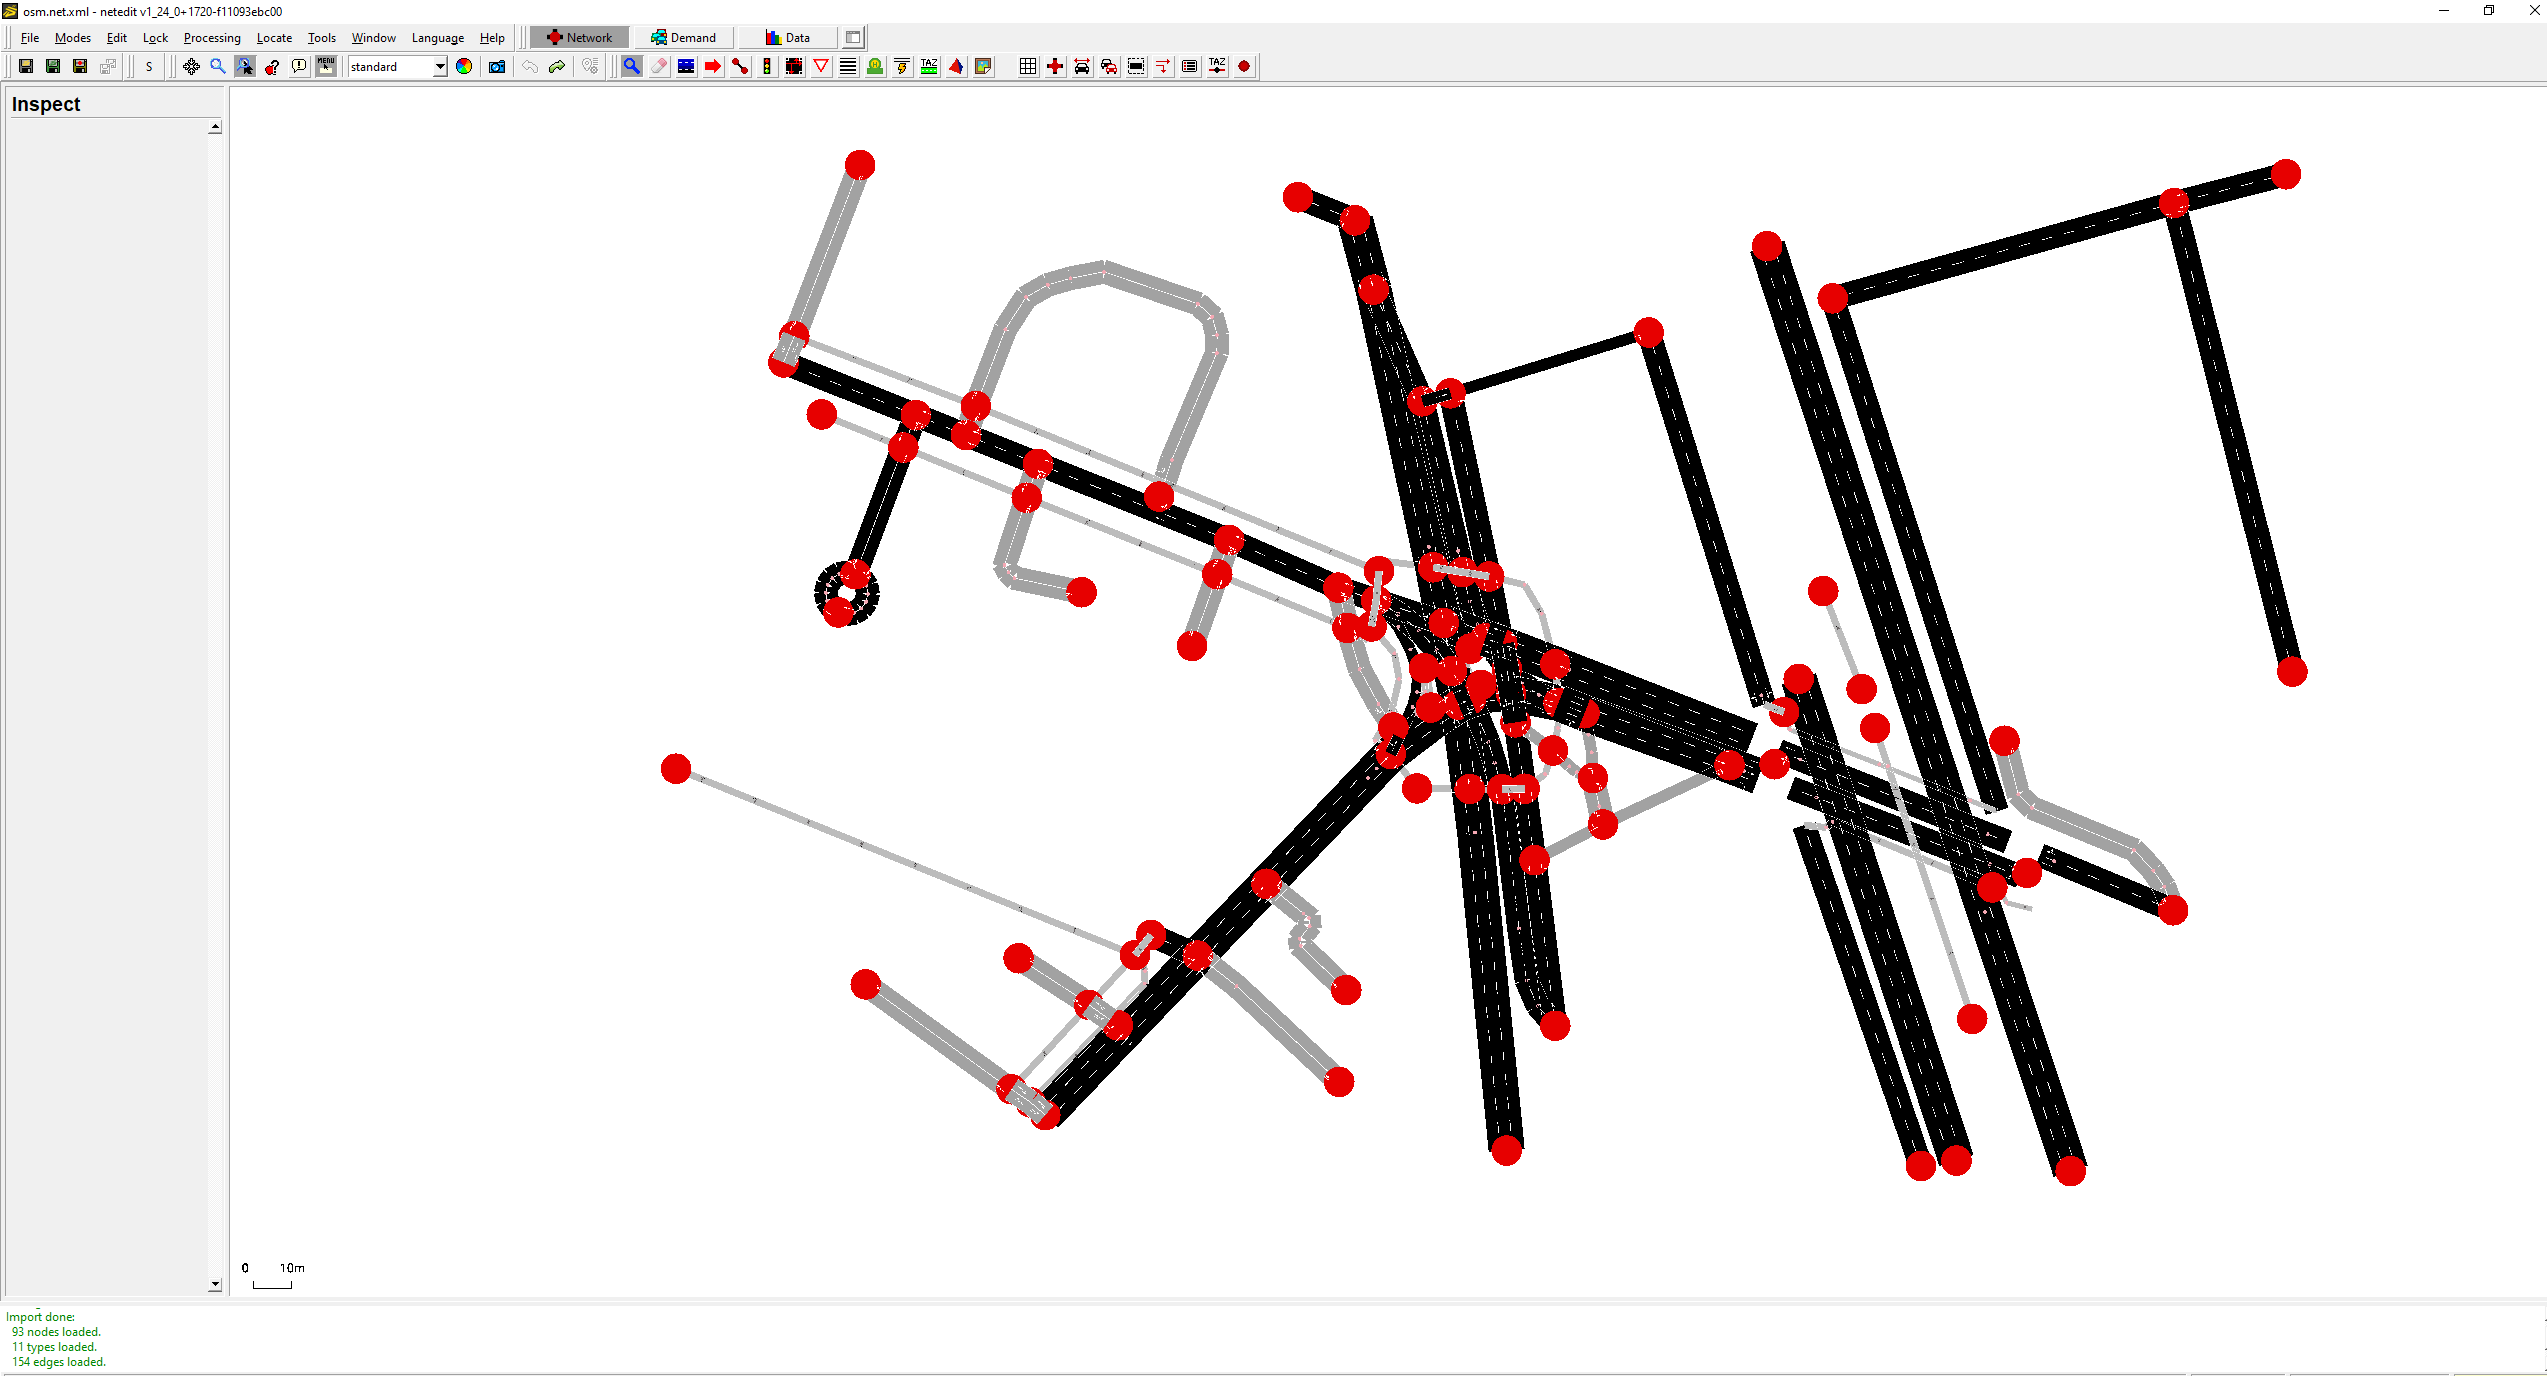
\includegraphics[width=0.48\textwidth]{NETEDIT.PNG}}
  \hfill
  \subfigure[Misma intersección tras la limpieza: calles irrelevantes
    eliminadas y sentidos de los carriles corregidos.]{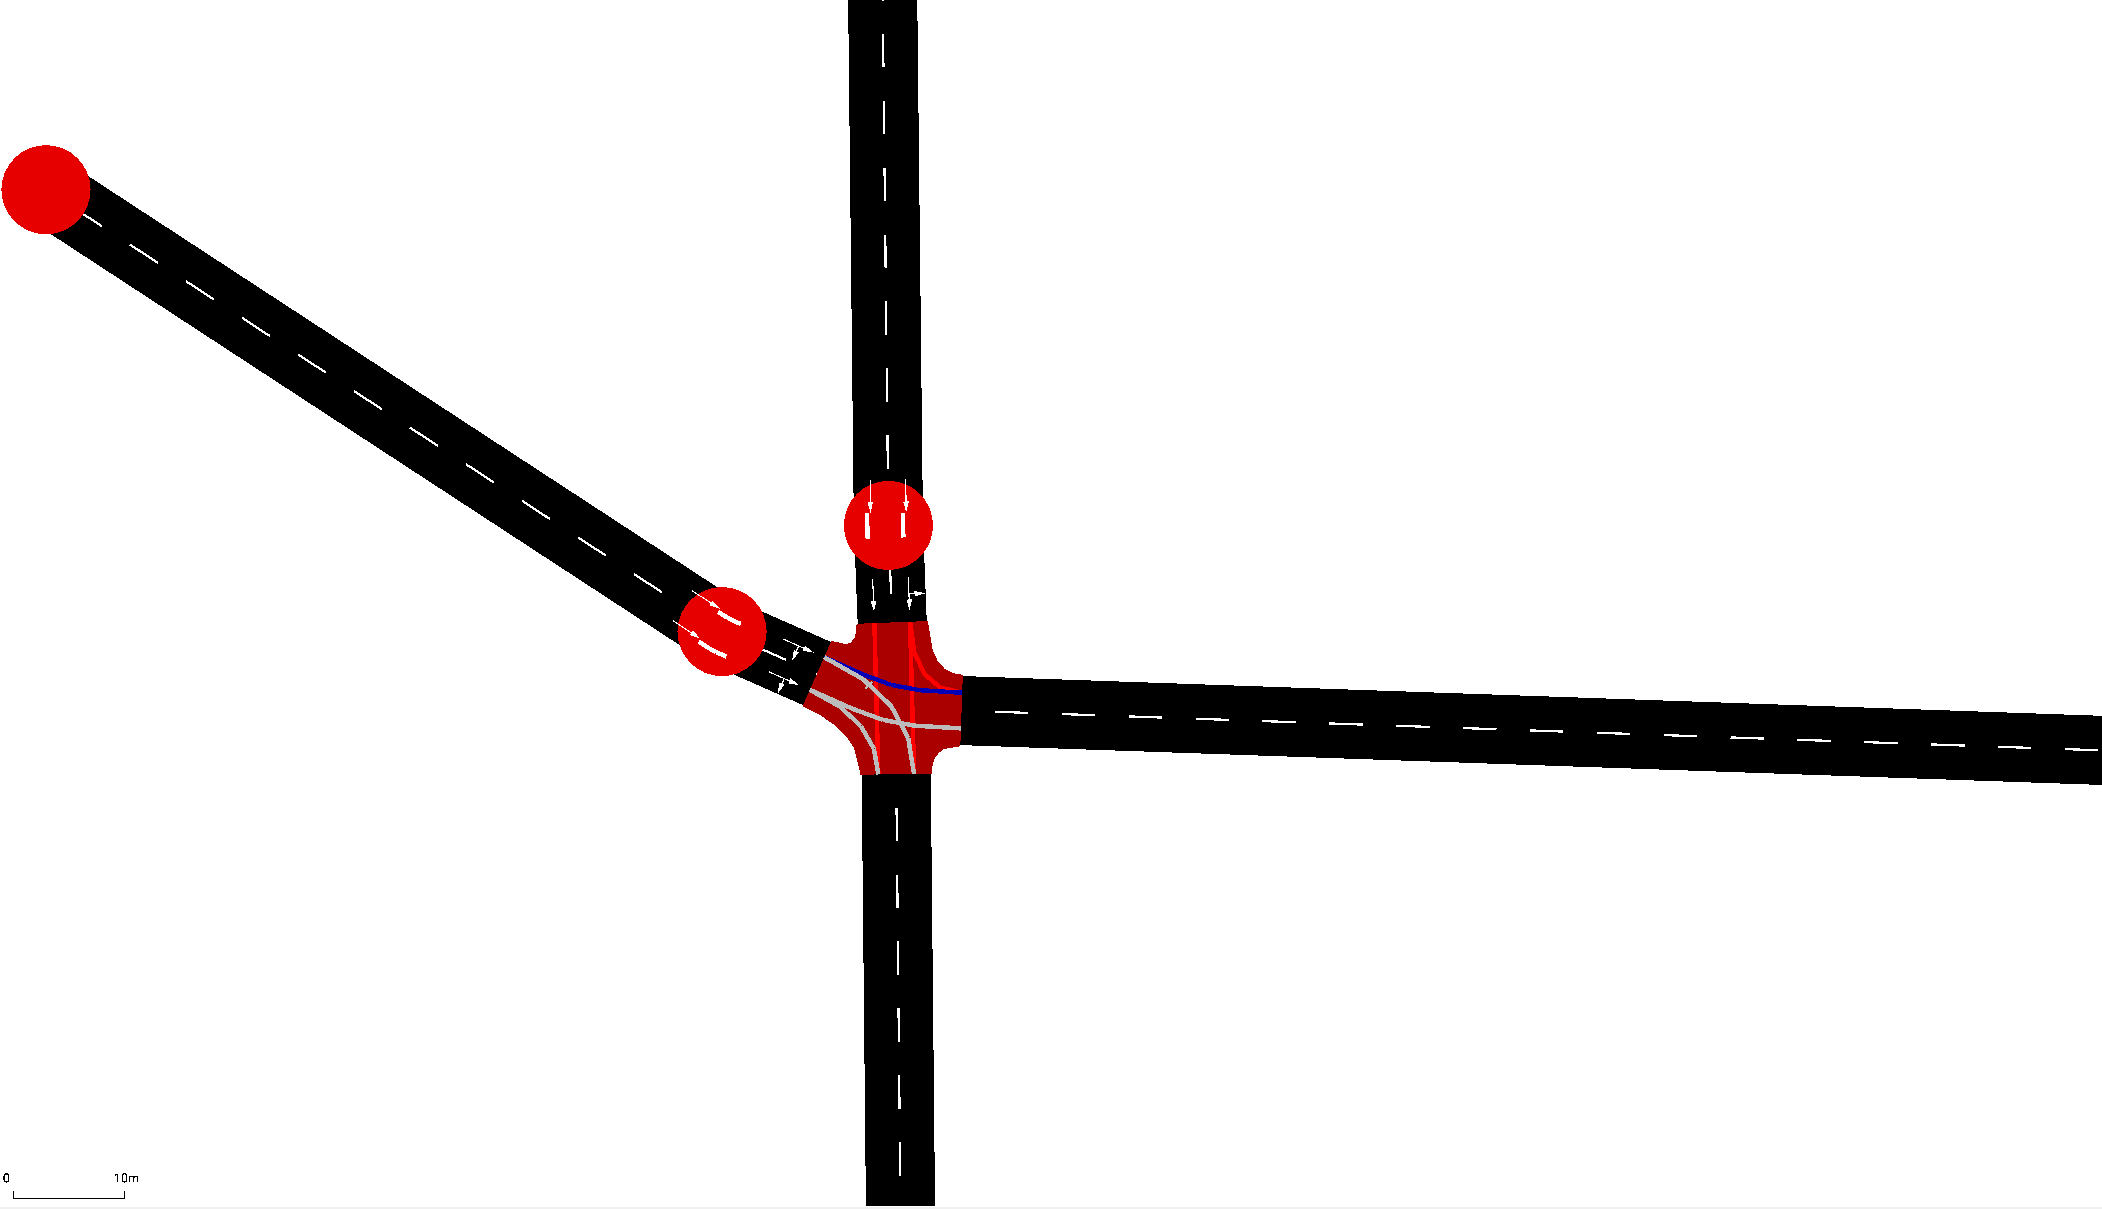
\includegraphics[width=0.48\textwidth]{conexiones.PNG}}
  \caption{Antes y después de la limpieza de la red en \texttt{netedit}, sobre una intersección de ejemplo importada desde OSM. Ilustra el procedimiento previsto para el cruce real de Lima; los escenarios evaluados en el Capítulo~\ref{cap:resultados} no provienen de OSM.}
  \label{fig:netedit-before-after}
\end{figure}


\subsection*{Herramientas útiles}

Para tareas de limpieza y configuración puede emplear las siguientes
herramientas que acompañan a SUMO:

\begin{itemize}
  \item \textbf{netconvert:} conversor de redes. Genera el
    \texttt{.net.xml} a partir de un recorte de OSM o de archivos de
    nodos, vías y conexiones escritos a mano, y es también donde se
    fijan los tiempos por omisión de los semáforos generados
    (\verb|--tls.green.time|, \verb|--tls.left-green.time|).
  \item \textbf{netedit:} editor gráfico que permite crear, modificar
    y depurar redes, así como editar semáforos, conexiones y
    restricciones de circulación. Resulta idóneo para eliminar
    segmentos irrelevantes y ajustar sentidos de vía tras una
    importación desde OSM.
  \item \textbf{sumo-gui:} interfaz gráfica de simulación que permite
    visualizar el comportamiento de los vehículos y los semáforos en
    tiempo real. Es útil para validar la red depurada y detectar
    cuellos de botella o comportamientos anómalos.
\end{itemize}


\section{Importación de un cruce desde OSM}

Para llevar al \textit{pipeline} una intersección real, el primer paso
es importar su cartografía. SUMO ofrece dos vías: el asistente gráfico
\emph{osmWebWizard}, que se describe a continuación, y la descarga
manual del recorte con \verb|osmGet.py| seguida de su conversión con
\verb|netconvert|, que da control más fino sobre los filtros de
importación a cambio de más pasos. Ambas producen el mismo tipo de
archivo \texttt{.net.xml} y requieren después la limpieza de la
Sección~\ref{sec:osm-limpieza}. Este procedimiento es el previsto para
el cruce de Lima y no se aplicó a los escenarios evaluados en esta
fase.

\subsection{Asistente OSM (\emph{osmWebWizard})}

\begin{enumerate}
  \item Ejecute el script \verb|osmWebWizard.py| desde la carpeta de
    herramientas de SUMO.  El script abre un navegador donde se puede
    navegar sobre el mapa de OSM, seleccionar la zona deseada y
    generar el escenario automáticamente.  El uso básico es:
    {\footnotesize\begin{verbatim}
python tools/osmWebWizard.py
    \end{verbatim}
    }

  \item Seleccione ``Lima, Peru'' en el buscador y ajuste el
    \emph{bounding box} sobre la intersección de interés.  Active la
    opción “Traffic lights” si desea que se importen los semáforos y
    pulse “Generate Scenario”.  El asistente creará la red
    \texttt{.net.xml}, una demanda aleatoria y un fichero
    \texttt{.sumocfg}; además iniciará \emph{sumo-gui} con el
    escenario resultante.  Los archivos se guardan en un
    subdirectorio con marca temporal.

  \item Revise la red en \emph{sumo-gui} y, si detecta calles
    desconectadas o giros imposibles, ajuste el recorte y repita la
    generación hasta obtener una red consistente.
\end{enumerate}

Para ilustrar este proceso, la Figura~\ref{fig:import-osm-sumo} muestra
la selección del área en OSM y la red generada en SUMO. A la
izquierda se observa el recuadro delimitado sobre el mapa en el asistente
\emph{osmWebWizard}, y a la derecha la red importada tal como aparece en
\emph{sumo-gui}.

\begin{figure}[H]
  \centering
  \subfigure[Selección del \textit{bounding box} en OSM mediante el
    asistente \emph{osmWebWizard}.]{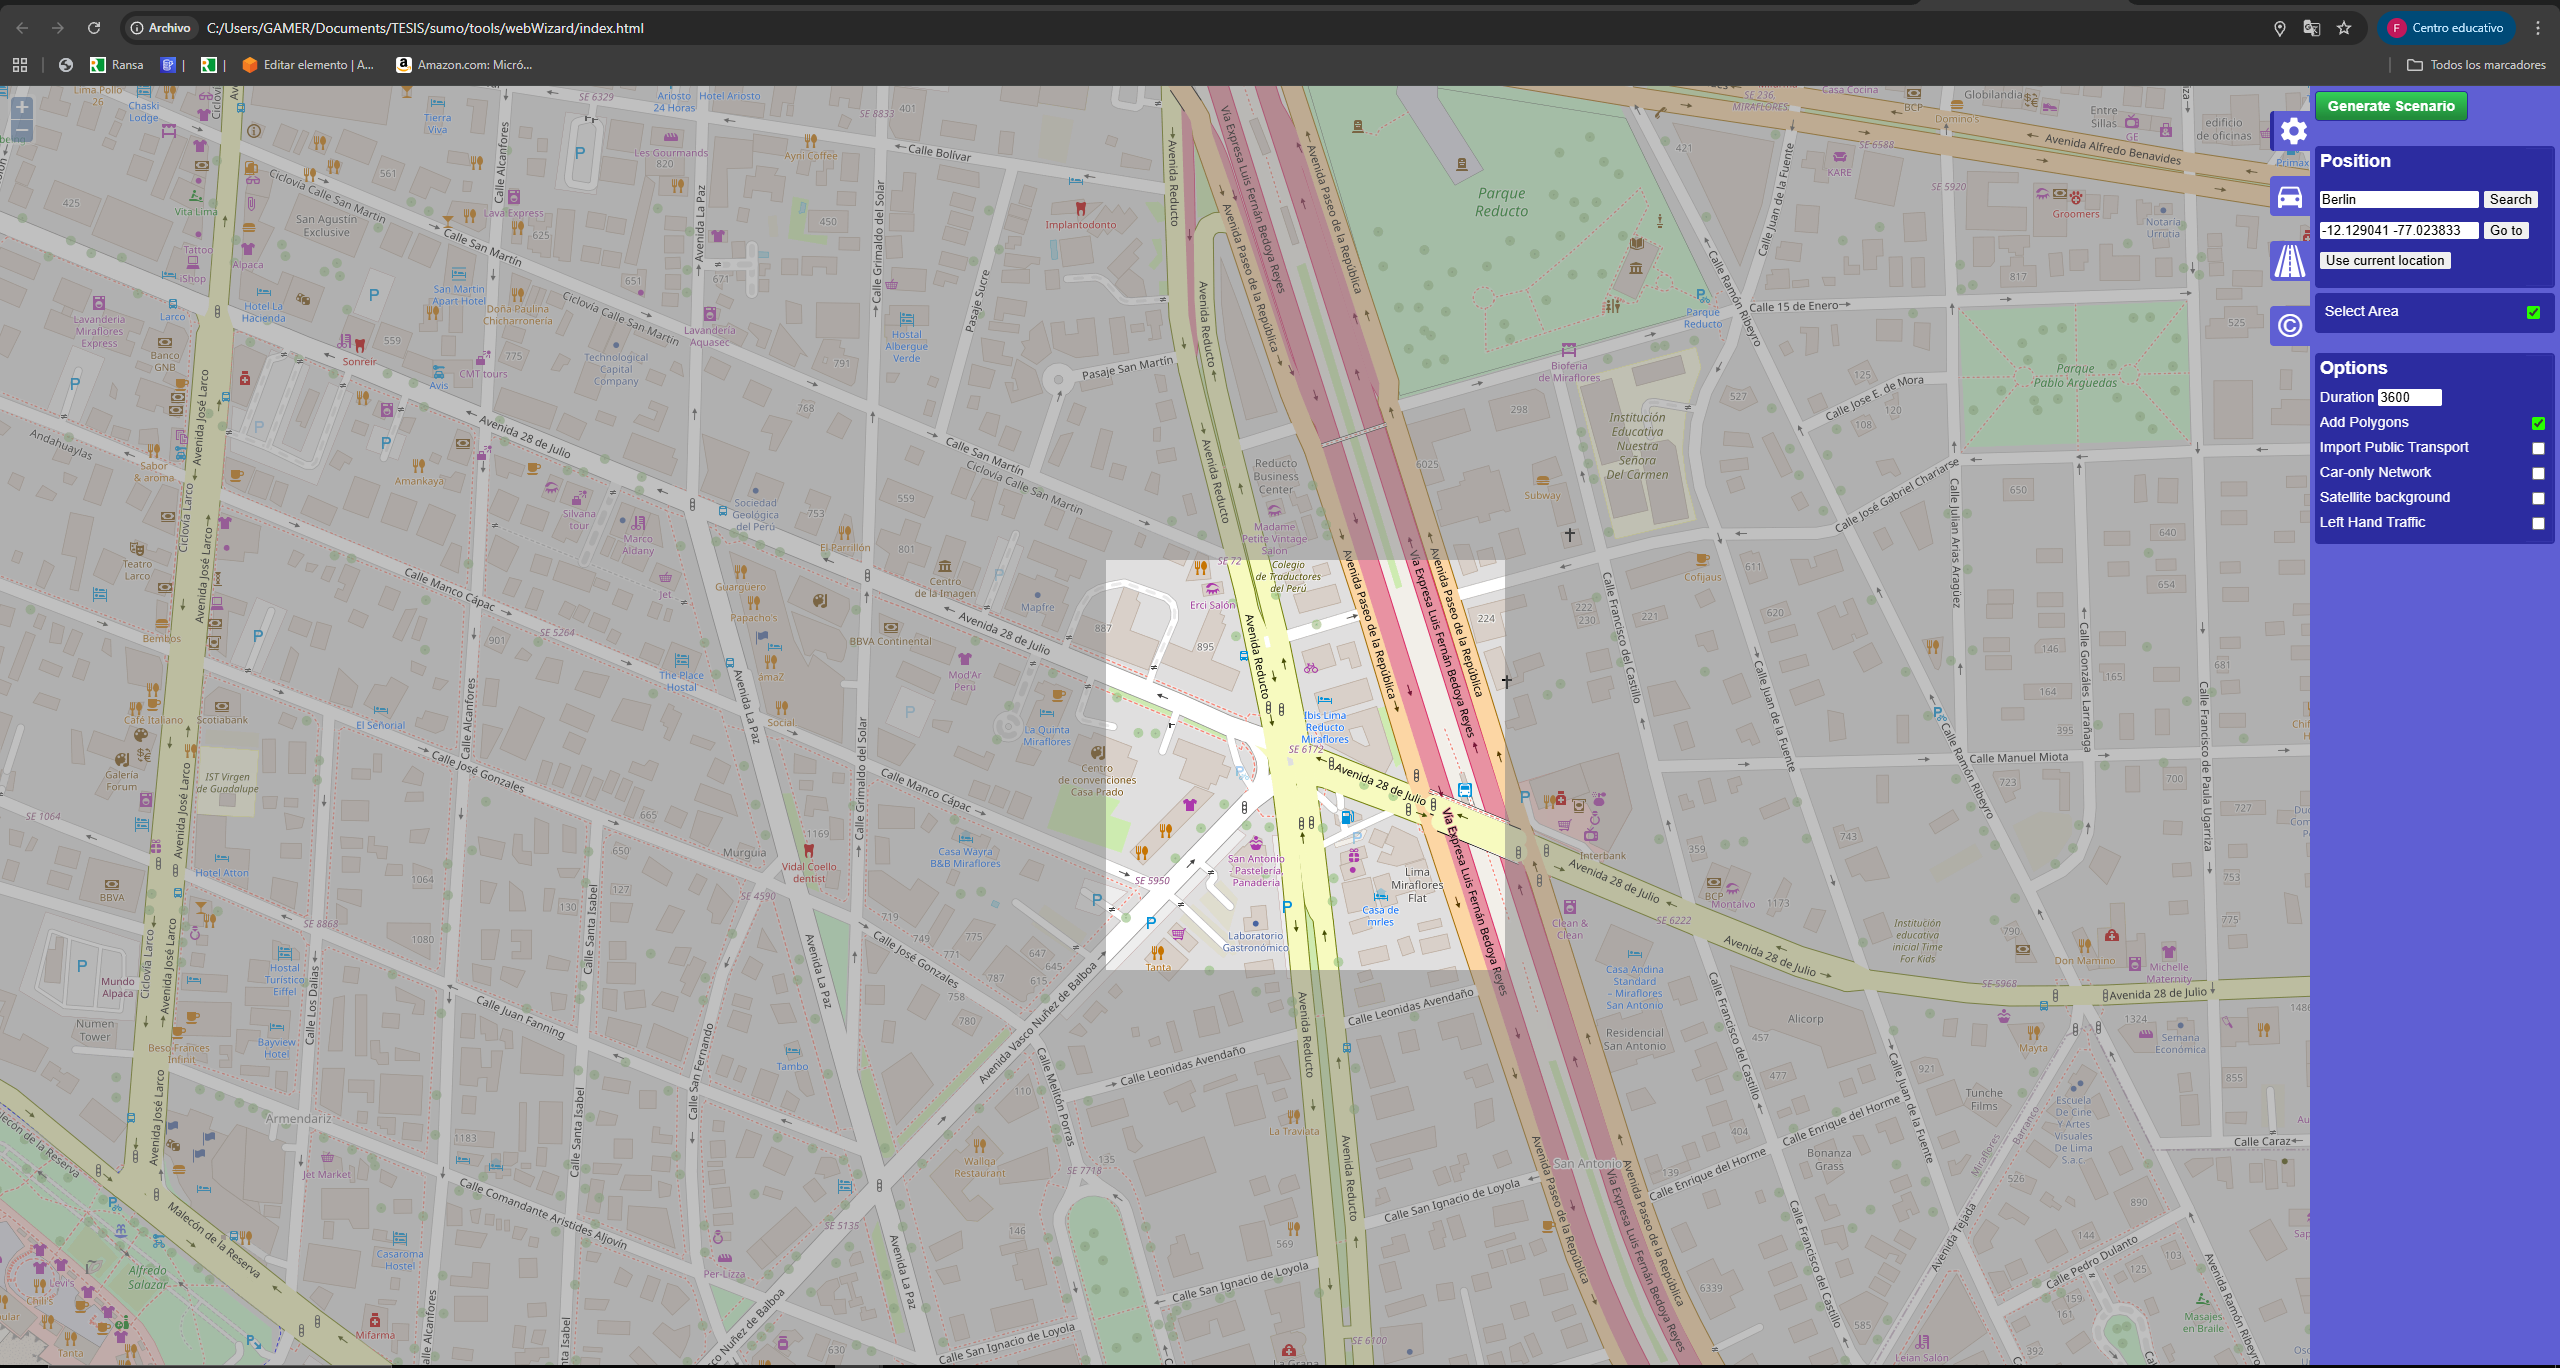
\includegraphics[width=0.48\textwidth]{OSM.PNG}}
  \hfill
  \subfigure[Red del cruce generada automáticamente en \emph{sumo-gui}.]{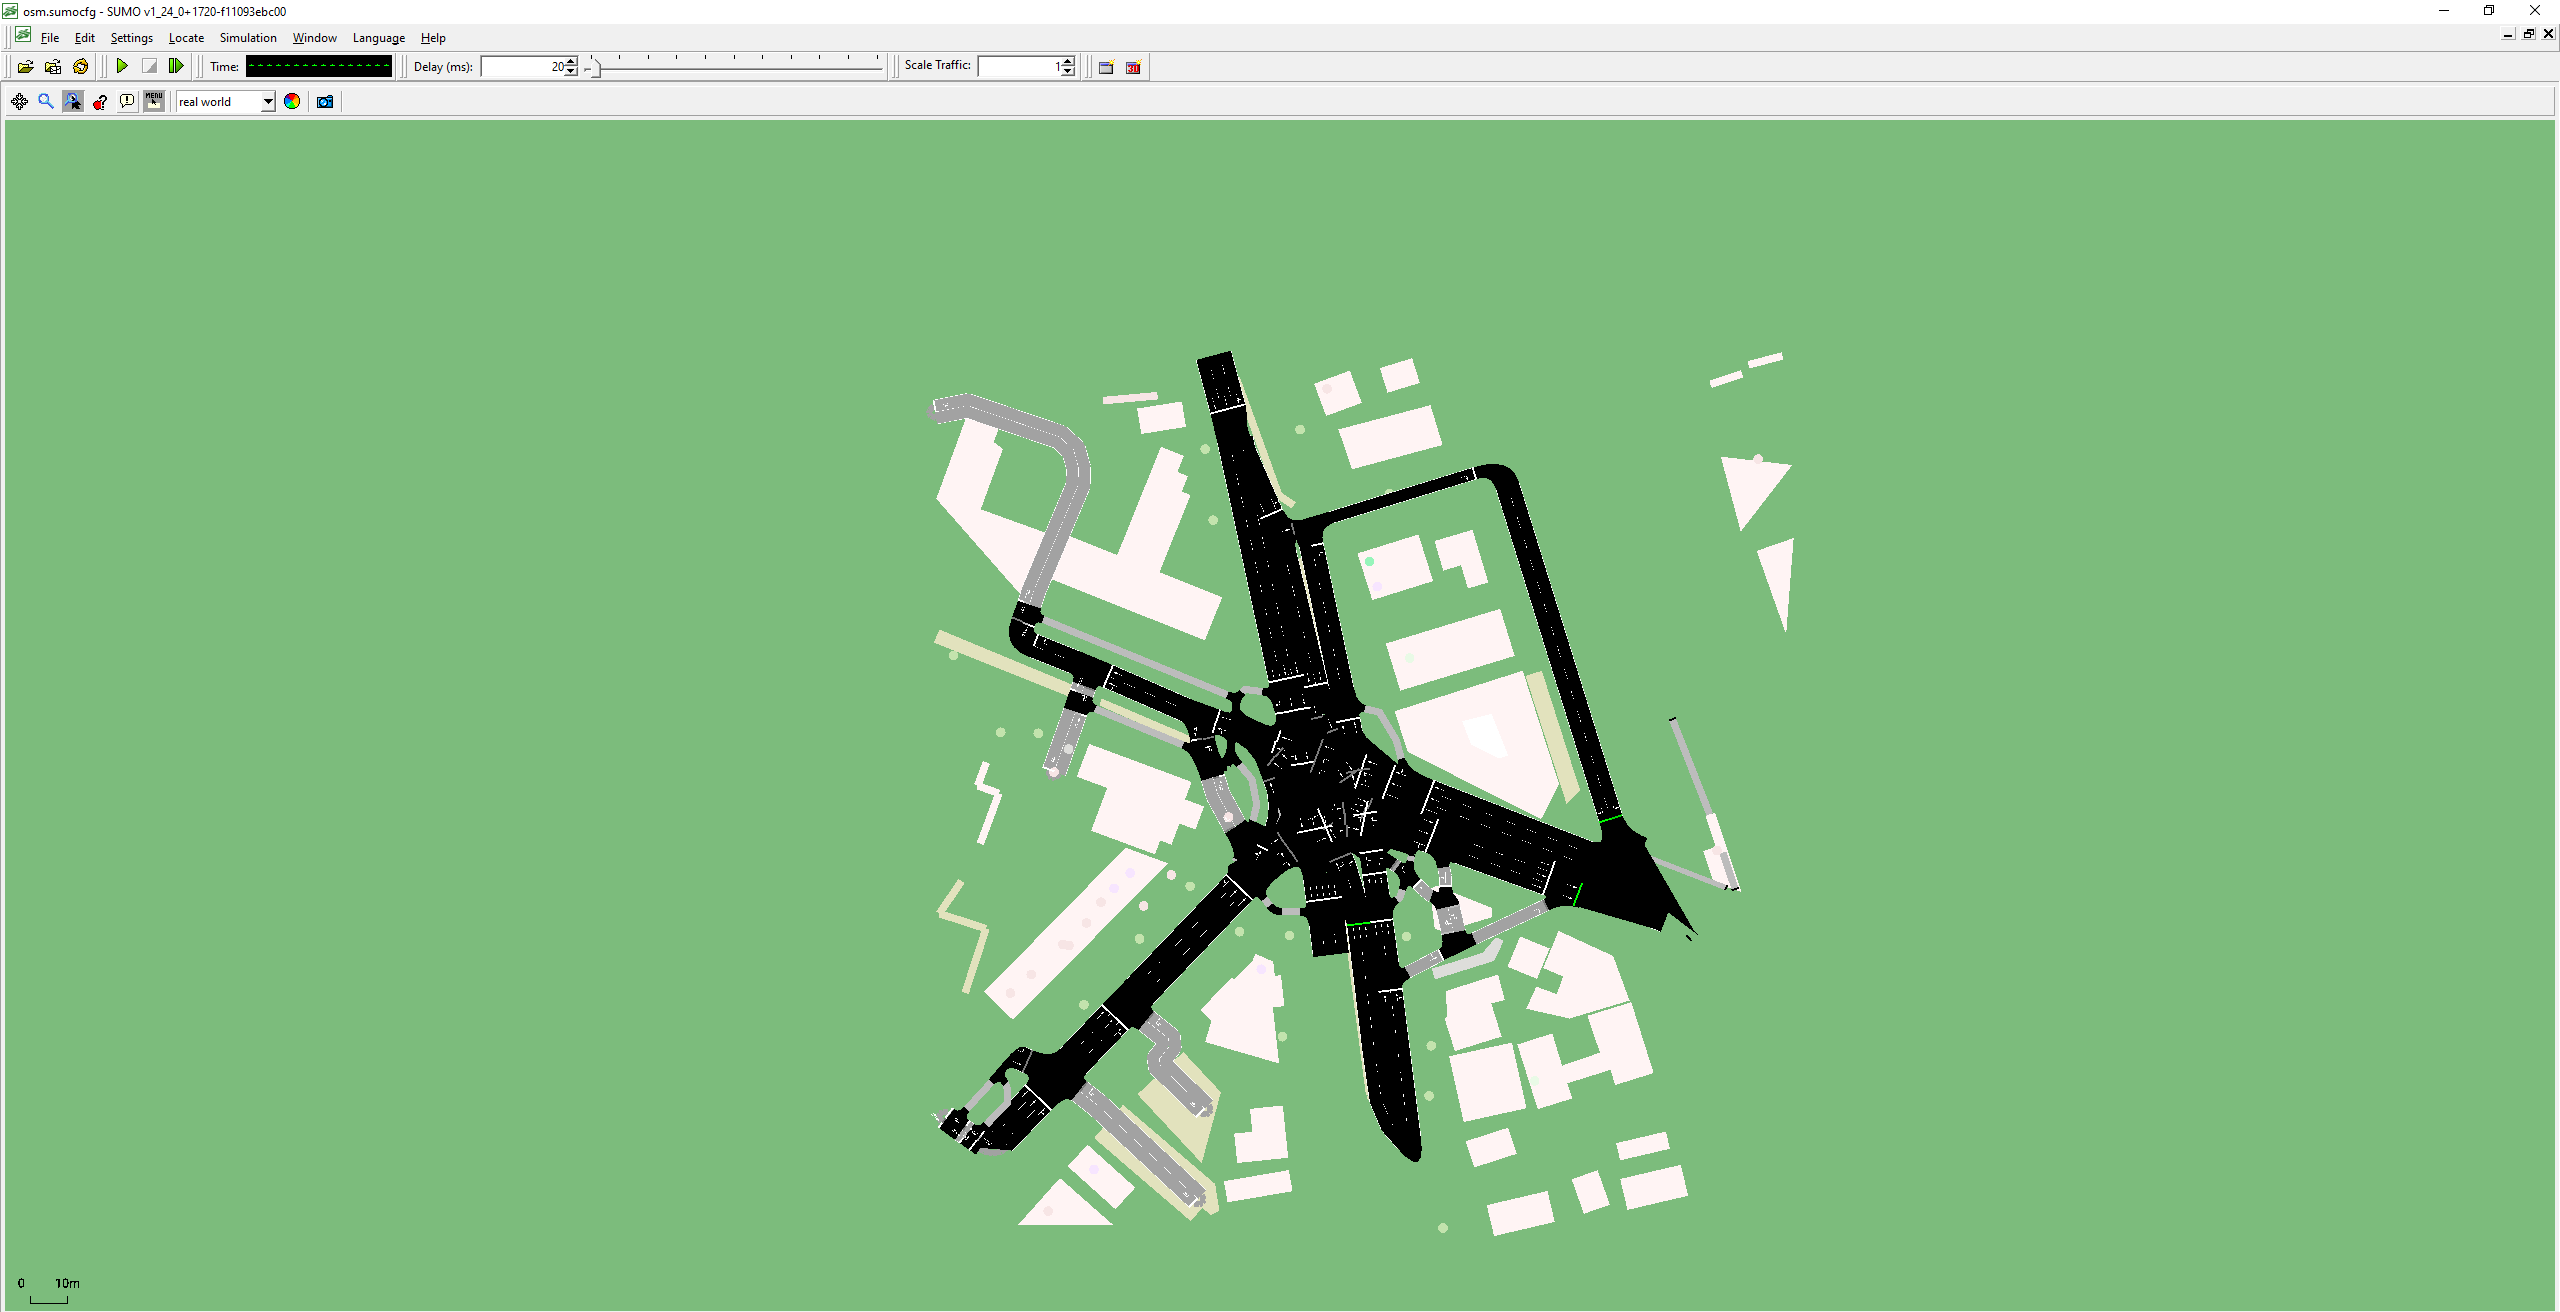
\includegraphics[width=0.48\textwidth]{SUMO.PNG}}
  \caption{Importación de un cruce desde OSM a SUMO mediante el asistente \emph{osmWebWizard}.}
  \label{fig:import-osm-sumo}
\end{figure}

\section{Diagrama de flujo del módulo U1}

La Figura~\ref{fig:flow-u1} resume el procedimiento completo del módulo U1,
desde la selección del cruce en Lima hasta la obtención del escenario SUMO
listo para ser utilizado en el entrenamiento del agente de RL (U2).

\begin{figure}[H]
    \centering
    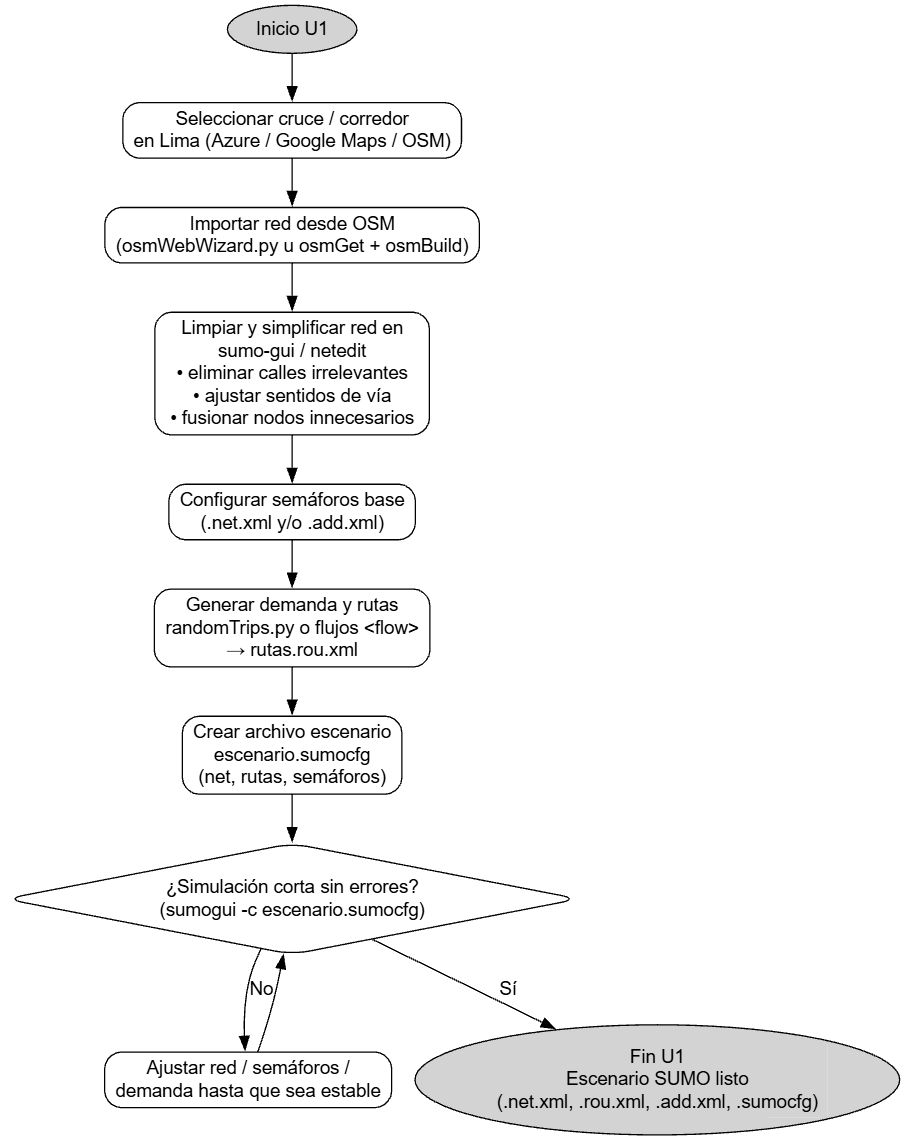
\includegraphics[width=\textwidth]{U1.png}
    \caption{Diagrama de flujo del módulo U1: preprocesamiento y generación del
    escenario SUMO.}
    \label{fig:flow-u1}
\end{figure}
